\documentclass{beamer}
\usetheme{Warsaw}
\setbeamertemplate{footline}[frame number]

\usepackage[utf8]{inputenc}
\usepackage{fancybox}
\usepackage{multimedia} 
\usepackage{subfig}
\usepackage{amsmath}
\usepackage{hyperref}
% Setze die Optionen für das hyperref-Paket
\hypersetup{
    colorlinks=true,    % Färbt die Links
    linkcolor=blue,     % Farbe für interne Links
    filecolor=magenta,  % Farbe für Links zu lokalen Dateien
    urlcolor=cyan,      % Farbe für externe Links
    pdftitle={Angewandte Mathematik}, % Titel des Dokuments
    pdfpagemode=FullScreen, % Öffnet das PDF im Vollbildmodus
}

\usepackage[all]{xy}
\begin{document}


\title[Angewandte Mathematik] % (optional, only for long titles)
{Angewandte Mathematik
\\
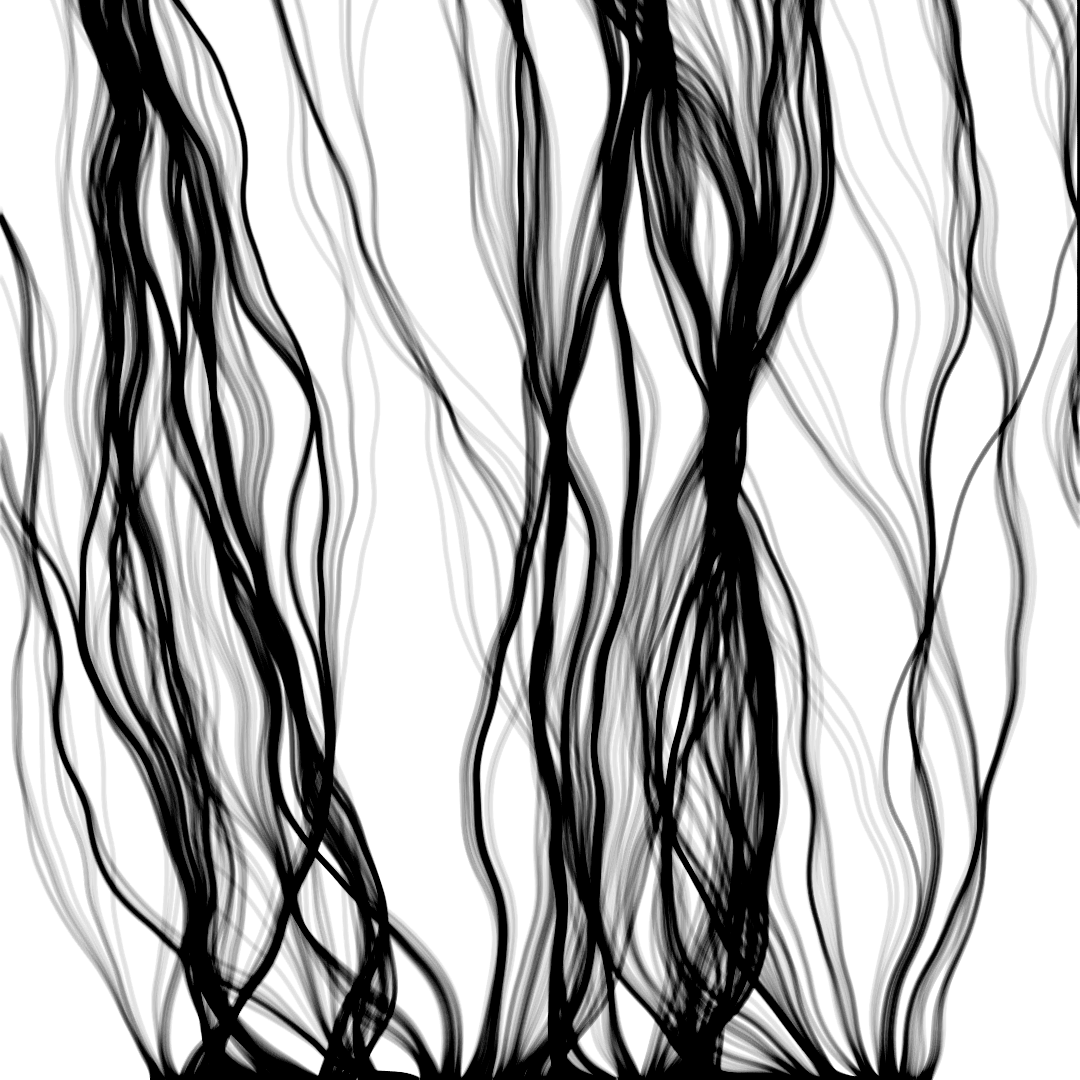
\includegraphics[scale=0.15]{images/cover}
}
\subtitle{}
\author[Dr. Johannes Riesterer] % (optional, for multiple authors)
{Dr.  rer. nat. Johannes Riesterer}

\date[KPT 2004] % (optional)
{}

\subject{Angewandte Mathematik}

\frame{\titlepage}






\begin{frame}
    \frametitle{Infinitessimalrechnung}
    \framesubtitle{Infinitessimalrechnung}
    \begin{block}{Sir Isaac Newton}
\begin{figure}[H]
      \centering
    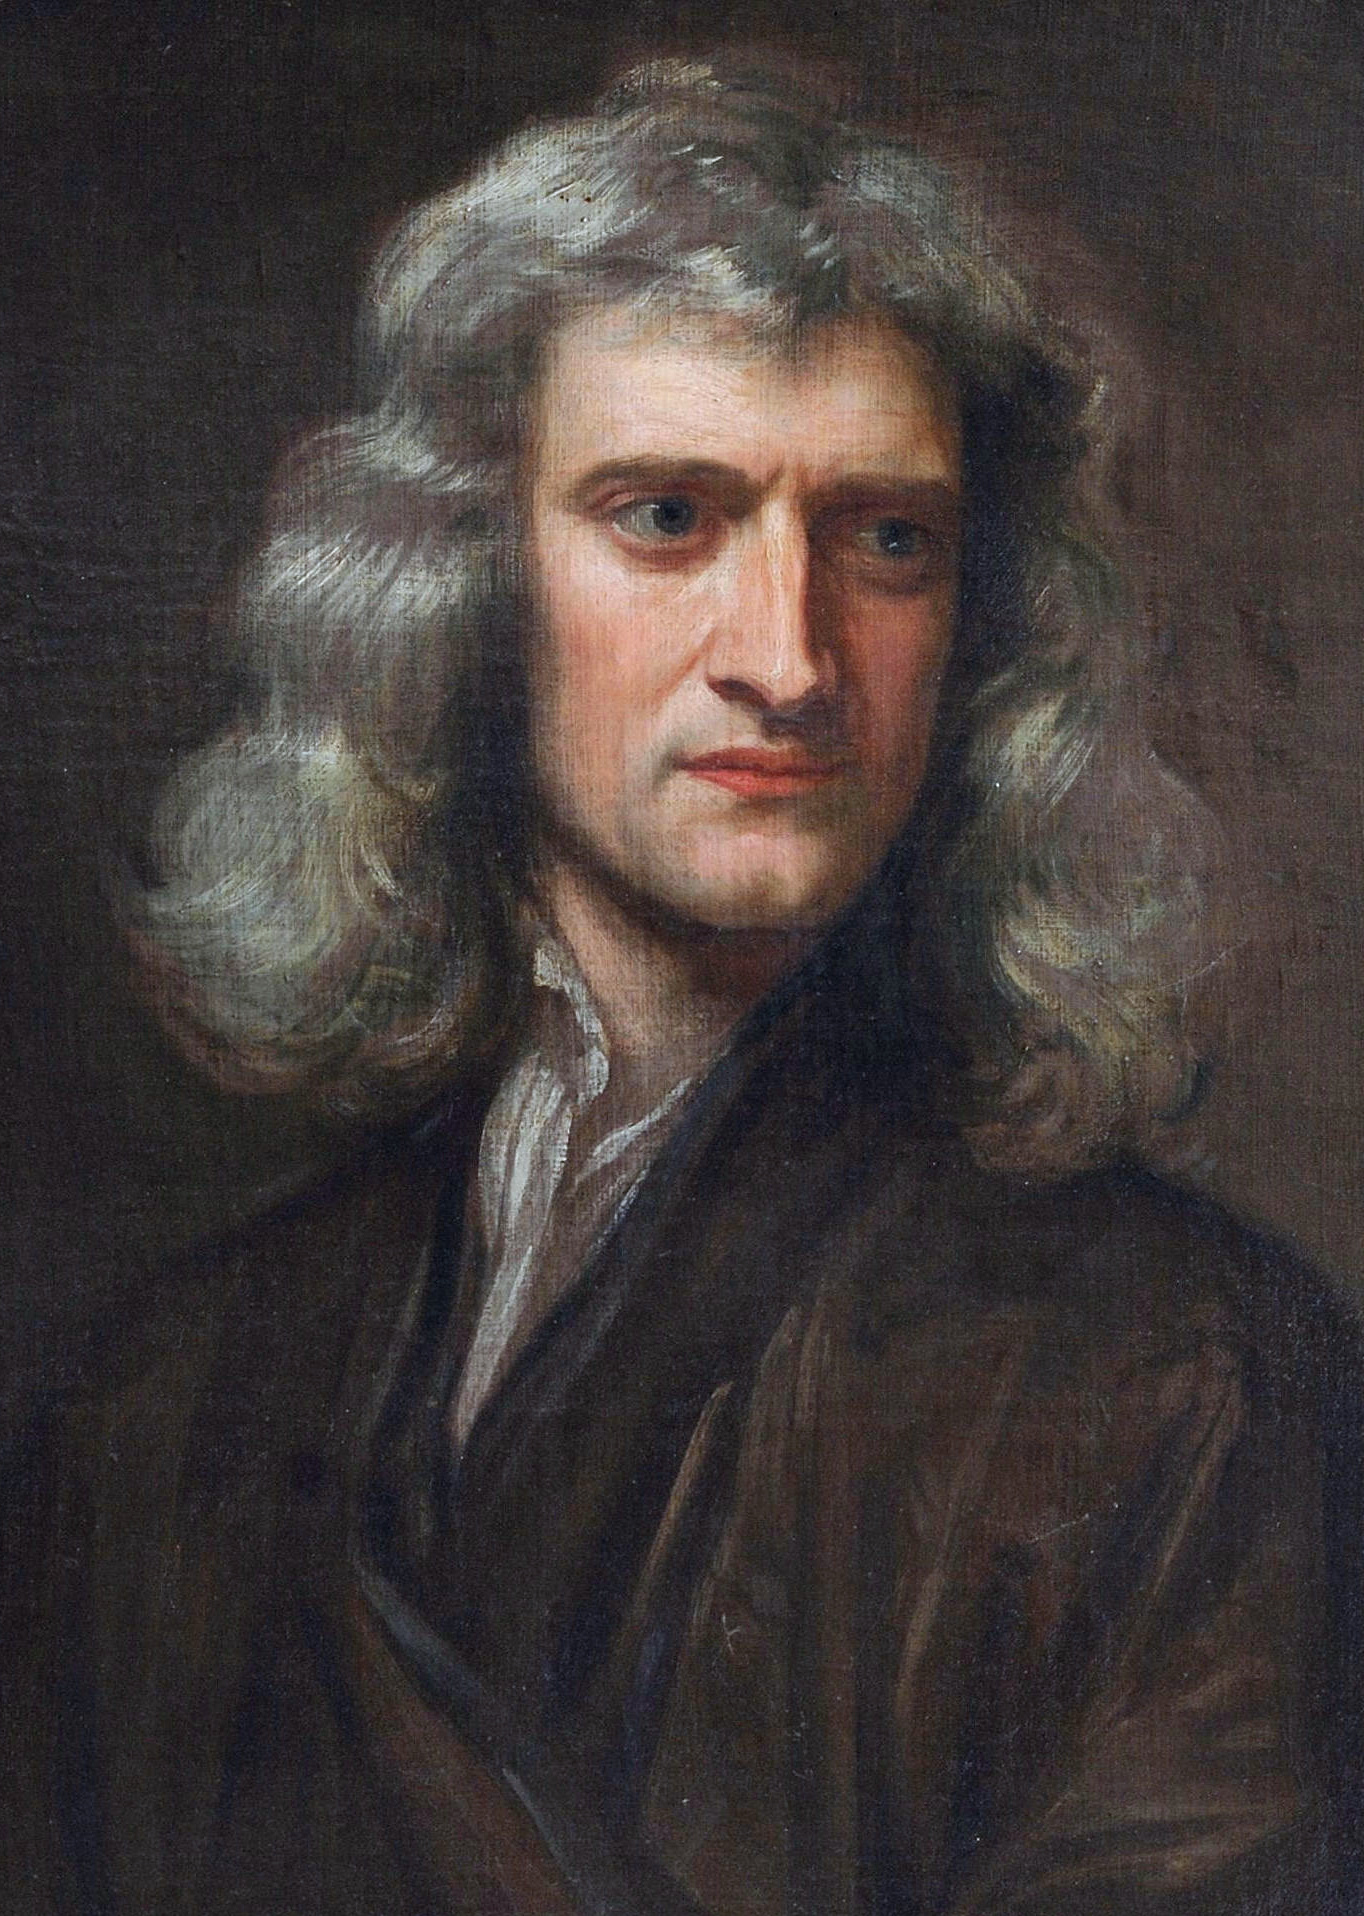
\includegraphics[width=0.4\textwidth]{images/Newton.jpg}
    %  \caption{Quelle: DALLE}
\end{figure}

\end{block}

 \end{frame}




 \begin{frame}
    \frametitle{Infinitessimalrechnung}
\framesubtitle{Infinitessimalrechnung}
    \begin{block}{Konvergenz erfahrungsgemäß}
Etwas  konvergiert gegen einen Grenzwert, 
wenn es sich diesem Grenzwert beliebig nahe annähert.
\end{block}

    \begin{figure}[H]
          \centering
        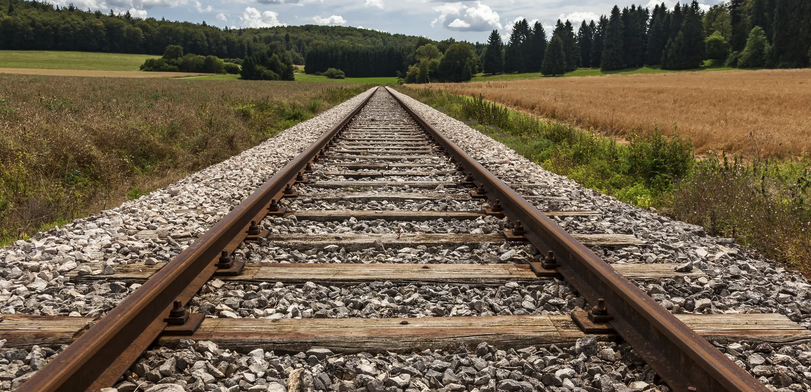
\includegraphics[width=0.8\textwidth]{images/limit}
          \caption{Konvergente Schienen}
    \end{figure}

\end{frame}


\begin{frame}
    \frametitle{Infinitessimalrechnung}
\framesubtitle{Infinitessimalrechnung}
    \begin{block}{Infinitessimalrechnung}
        Wie kann man damit rechnen und braucht man das?
\end{block}
 \end{frame}


 \begin{frame}
    \frametitle{Infinitessimalrechnung}
\framesubtitle{Limes}
    \begin{block}{Achilles und die Schildkröte}
\begin{figure}[H]
      \centering
    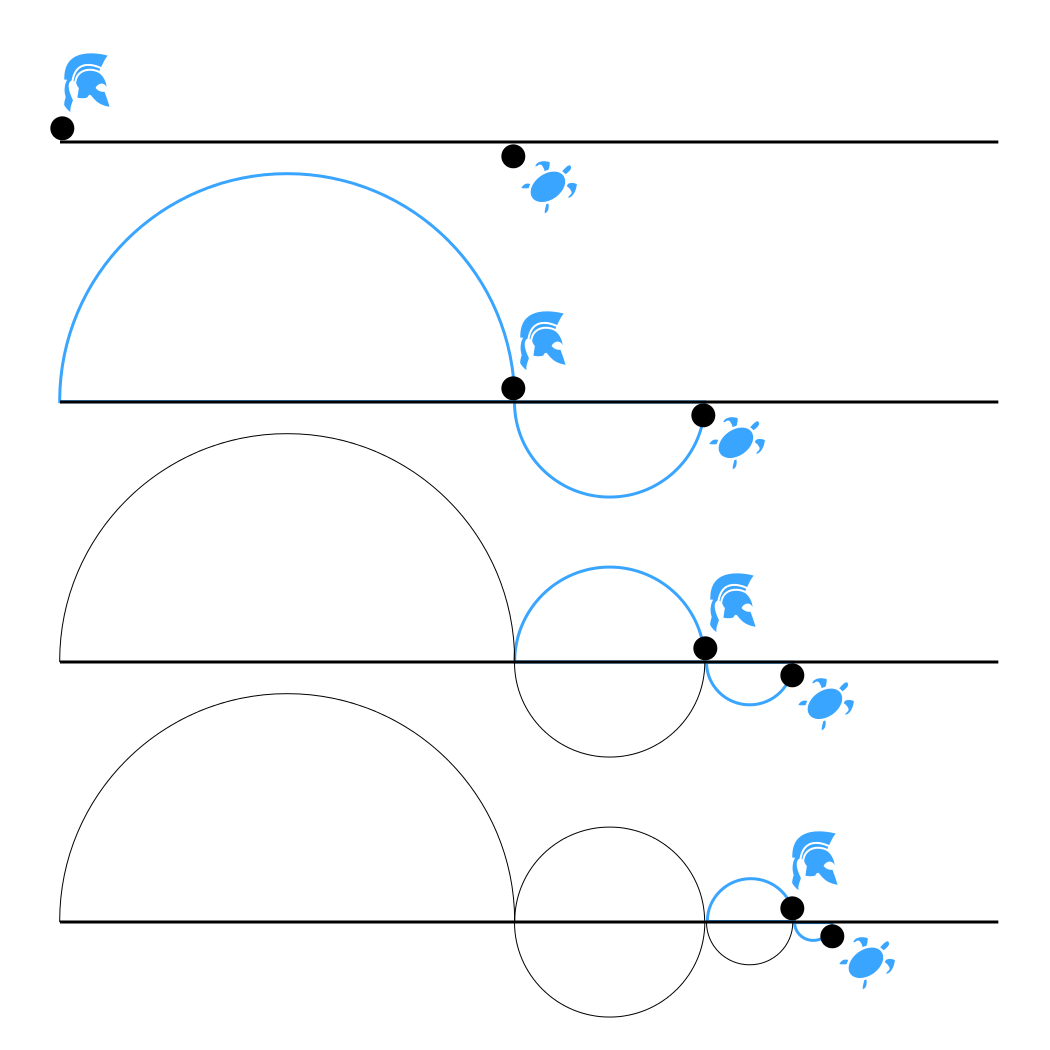
\includegraphics[width=0.3\textwidth]{images/Zeno_Achilles_Paradox}
      \caption{Quelle: Wikipedia: }
\end{figure}
\href{https://www.youtube.com/watch?v=X8Qksx_Ng9k}{Mehr hier im Video}
\end{block}
  \begin{block}{Paradoxon der Antike}
 Obwohl Achilles schneller ist, kann er die Schildkröte niemals einholen.
\end{block}
 \end{frame}


\begin{frame}
    \frametitle{Infinitessimalrechnung}
\framesubtitle{Limes}
    \begin{block}{Achilles und die Schildkröte infinitessimal betrachtet}
Sei $s_0$ der Vorsprung der Schildkröte zu Beginn des Rennens, $t_0$ die Zeit, die Achilles benötigt, um $s_0$ zurückzulegen. Die Schildkröte sei $q$-mal langsamer als Achilles.
Dann ist Achilles  bei der Zeit $t_0 \cdot q$ ein weiteres Mal dort, wo die Schidlkröte vorher war. 
Nach der Zeit $(t_0 \cdot q) \cdot q = t_0 \cdot q^2$ ein drittes Mal usw.
Mit $q^0 = 1$ ist die Summe aller betrachteten Zeiten, die Achilles zurücklegt:

$t = t_0 \cdot \sum_{n=0}^\infty q^n = t_0 \cdot \lim_{n \to \infty} \sum_{k=0}^{n} q^{k} = t_0 \cdot \lim_{n \to \infty} \frac{1 - q^{n+1}}{1 -q} = \frac{t_0}{1 -q}$.
\end{block}
 \end{frame}






\begin{frame}
    \frametitle{Infinitessimalrechnung}
\framesubtitle{Limes}

\begin{block}{Folge}
    Eine reelle Folge ist eine Abbildung
    \begin{align*}
    a: \mathbb{N} \rightarrow \mathbb{R}^n
    \end{align*}
 Für $n \in \mathbb{N}$ bezeichnen wir $a_n := a(n)$ als $n$ tes Folgenglied.
\end{block}


 \end{frame}



 \begin{frame}
    \frametitle{Infinitessimalrechnung}
\framesubtitle{Limes}

\begin{block}{Konvergenz}
    Eine Folge $a_n$ in $\mathbb{R}^n$ heißt konvergent gegen den Grenzwert $a \in \mathbb{R}^n$, wenn gilt:
    \begin{align*}
    \forall {\varepsilon > 0} \ \exists \ N \in \mathbb{N} \; \forall \ n > N: \; d(a, a_n) < \varepsilon\,
    \end{align*}
    in Worten: Es gibt für jedes beliebige (noch so kleine) $\varepsilon$ einen Index $N$ derart, dass für alle Indizes $n > N$, alle weiteren Folgenglieder, gilt: der Abstand $d(a, a_n)$ ist kleiner als $\varepsilon$.
    \end{block}


\begin{figure}[H]
      \centering
    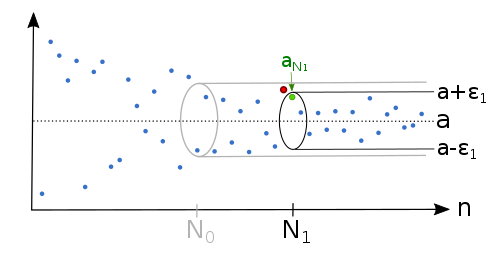
\includegraphics[width=0.7\textwidth]{images/500px-Epsilonschlauch_klein}
      \caption{Quelle: Wikipedia: https://commons.wikimedia.org/wiki/File:Epsilonschlauch\_klein.svg}
\end{figure}

 \end{frame}




\begin{frame}{Axiome eines metrischen Raumes}
    Ein metrischer Raum ist ein Paar \((X, d)\), wobei \( X \) eine Menge und \( d: X \times X \rightarrow \mathbb{R} \) eine Abbildung ist, die die folgenden Axiome erfüllt:
    \begin{itemize}
      \item \textbf{Nichtnegativität}: \( d(x, y) \geq 0 \quad \forall x, y \in X \).
      \item \textbf{Identität der Ununterscheidbaren}: \( d(x, y) = 0 \) genau dann, wenn \( x = y \).
      \item \textbf{Symmetrie}: \( d(x, y) = d(y, x) \quad \forall x, y \in X \).
      \item \textbf{Dreiecksungleichung}: \( d(x, z) \leq d(x, y) + d(y, z) \quad \forall x, y, z \in X \).
    \end{itemize}
  \end{frame}
  
  \begin{frame}{Beispiel eines metrischen Raumes}
    Betrachte den Raum \( \mathbb{R} \) mit der absoluten Differenz als Metrik:
    \[
    d(x, y) = |x - y|, \quad \forall x, y \in \mathbb{R}.
    \]
    Überprüfung der Axiome:
    \begin{itemize}
      \item \textbf{Nichtnegativität}: \( |x - y| \geq 0 \).
      \item \textbf{Identität der Ununterscheidbaren}: \( |x - y| = 0 \) genau dann, wenn \( x = y \).
      \item \textbf{Symmetrie}: \( |x - y| = |y - x| \).
      \item \textbf{Dreiecksungleichung}: \( |x - z| \leq |x - y| + |y - z| \).
    \end{itemize}
  \end{frame}
  

  \begin{frame}{Normen in einem Vektorraum}
    Sei \( X = \mathbb{R}^n \) ein Vektorraum. Eine Norm auf \( X \) ist eine Abbildung \( \| \cdot \| : X \rightarrow \mathbb{R} \), 
    die für alle \( x, y \in X \) und \( \alpha \in \mathbb{R} \) folgende Eigenschaften erfüllt:
    \begin{itemize}
      \item \textbf{Positive Definitheit}: \( \|x\| \geq 0 \) und \( \|x\| = 0 \) genau dann, wenn \( x = 0 \).
      \item \textbf{Homogenität}: \( \|\alpha x\| = |\alpha| \cdot \|x\| \).
      \item \textbf{Dreiecksungleichung}: \( \|x + y\| \leq \|x\| + \|y\| \).
    \end{itemize}
  
    \vspace{0.5cm}
    \textbf{Beispiel: Euklidische Norm in \( \mathbb{R}^2 \)}
  
    Sei \( x = (x_1, x_2) \in \mathbb{R}^2 \). Dann ist die euklidische Norm gegeben durch:
    \[
    \|x\|_2 = \sqrt{x_1^2 + x_2^2}.
    \]
  
    \textbf{Konkretes Beispiel:} Für \( x = (3, 4) \) gilt:
    \[
    \|x\|_2 = \sqrt{3^2 + 4^2} = \sqrt{9 + 16} = \sqrt{25} = 5.
    \]
  \end{frame}
  

  \begin{frame}{Abstände durch Normen}
    Sei \( X = \mathbb{R}^n \)  ein Vektorraum und \( \| \cdot \| : X \rightarrow \mathbb{R} \) eine Norm. Ein durch die Norm definierter Abstand ist gegeben durch:
    \[
    d(x, y) = \| x - y \|,
    \]
    wobei \( x, y \in X \) beliebige Punkte sind. Dieser Abstand erfüllt die Axiome eines metrischen Raumes:
    \begin{itemize}
      \item \textbf{Nichtnegativität}: \( d(x, y) = \| x - y \| \geq 0 \).
      \item \textbf{Identität der Ununterscheidbaren}: \( d(x, y) = 0 \) genau dann, wenn \( x = y \).
      \item \textbf{Symmetrie}: \( d(x, y) = \| x - y \| = \| y - x \| = d(y, x) \).
      \item \textbf{Dreiecksungleichung}: \( \| x - z \| \leq \| x - y \| + \| y - z \| \quad \forall x, y, z \in X \).
    \end{itemize}
    \textbf{Beispiele:}
    \begin{itemize}
      \item \textbf{Euklidische Norm:} \( \| x \|_2 = \sqrt{\sum_{i=1}^{n} |x_i|^2} \).
      \item \textbf{Manhattan-Norm:} \( \| x \|_1 = \sum_{i=1}^{n} |x_i| \).
      \item \textbf{Maximum-Norm:} \( \| x \|_\infty = \max_{1 \leq i \leq n} |x_i| \).
    \end{itemize}
  \end{frame}


  
  \begin{frame}{Skalarprodukt}
      \textbf{Definition:} \\
      Ein Skalarprodukt ist eine Abbildung 
      \[
      \langle \cdot, \cdot \rangle: V \times V \to \mathbb{R}
      \]
      auf einem reellen Vektorraum \( V \), die folgende Eigenschaften erfüllt:
      \begin{itemize}
          \item \textbf{Linearität:} \( \langle a \mathbf{v} + b \mathbf{w}, \mathbf{u} \rangle = a \langle \mathbf{v}, \mathbf{u} \rangle + b \langle \mathbf{w}, \mathbf{u} \rangle \)
          \item \textbf{Symmetrie:} \( \langle \mathbf{v}, \mathbf{u} \rangle = \langle \mathbf{u}, \mathbf{v} \rangle \)
          \item \textbf{Positivität:} \( \langle \mathbf{v}, \mathbf{v} \rangle \geq 0 \) und \( \langle \mathbf{v}, \mathbf{v} \rangle = 0 \) genau dann, wenn \( \mathbf{v} = 0 \)
      \end{itemize}
  \end{frame}
  
  \begin{frame}{Euklidisches Skalarprodukt}
      \textbf{Beispiel: Euklidisches Skalarprodukt} \\
      In \( \mathbb{R}^n \) ist das Skalarprodukt definiert als:
      \[
      \langle \mathbf{v}, \mathbf{w} \rangle = \sum_{i=1}^n v_i w_i
      \]
      für \( \mathbf{v} = (v_1, v_2, \dots, v_n) \) und \( \mathbf{w} = (w_1, w_2, \dots, w_n) \).
  \end{frame}
  
  \begin{frame}{Zusammenhang mit der Norm}
      \textbf{Definition:} \\
      Die durch das Skalarprodukt induzierte Norm ist definiert als:
      \[
      \|\mathbf{v}\| = \sqrt{\langle \mathbf{v}, \mathbf{v} \rangle}
      \]
      \textbf{Beispiel: Euklidische Norm} \\
      Für das euklidische Skalarprodukt ist die Norm:
      \[
      \|\mathbf{v}\| = \sqrt{\sum_{i=1}^n v_i^2}
      \]
      Diese Norm wird auch als \textit{Euklidische Norm} oder \textit{2-Norm} bezeichnet.
  \end{frame}
  


  \begin{frame}
    
    \frametitle{Definition: Topologischer Raum }
    \begin{block}{Topologischer Raum \href{https://github.com/leanprover-community/mathlib4/blob/418a5eb7aec3fb639097cb13f74fc031ac4057f2/Mathlib/Topology/Defs/Basic.lean\#L61-L71}{Mathlib}}
    Ein \emph{topologischer Raum} ist ein Paar $(X, \mathcal{T})$, wobei $X$ eine Menge und $\mathcal{T}$ eine Familie von Teilmengen von $X$ ist, die folgende Eigenschaften erfüllt:
    \begin{enumerate}
        \item $\emptyset \in \mathcal{T}$ und $X \in \mathcal{T}$ (Die leere Menge und die Gesamtheit $X$ gehören zur Topologie).
        \item Wenn $A, B \in \mathcal{T}$, dann gilt $A \cap B \in \mathcal{T}$ (Schnittstabilität von endlichen Mengen).
        \item Wenn $\{A_i\}_{i \in I}$ eine beliebige Familie von Mengen in $\mathcal{T}$ ist, dann gilt $\bigcup_{i \in I} A_i \in \mathcal{T}$ (Vereinigungsstabilität von beliebigen Mengen).
    \end{enumerate}
    Die Familie $\mathcal{T}$ heißt die \emph{Topologie} auf der Menge $X$. Die Mengen in $\mathcal{T}$ werden als \emph{offene Mengen} bezeichnet.
\end{block}           
  \end{frame}


% Folie 2: Beispiel: Standardtopologie durch den Abstand
\begin{frame}
    \frametitle{Beispiel: Standardtopologie durch den Abstand}
    Sei $(X, d)$ ein \emph{metrischer Raum} mit Abstandsfunktion $d: X \times X \rightarrow \mathbb{R}_{\geq 0}$.
    Die \emph{Standardtopologie} $\mathcal{T}_d$ auf $X$ wird durch den Abstand $d$ induziert, indem als offene Mengen die folgenden Teilmengen $U \subseteq X$ gewählt werden:
    \[
    U \in \mathcal{T}_d \quad \Leftrightarrow \quad \forall x \in U, \; \exists \epsilon > 0 \; \text{sodass} \; B_\epsilon(x) \subseteq U,
    \]
    wobei $B_\epsilon(x) = \{ y \in X \mid d(x, y) < \epsilon \}$ eine \emph{offene Kugel} um den Punkt $x$ mit Radius $\epsilon$ ist.
\end{frame}




% Folie 1: Definition eines Filters
\begin{frame}
    \frametitle{Definition: Filter }
    \begin{block}{Filter \href{https://github.com/leanprover-community/mathlib4/blob/418a5eb7aec3fb639097cb13f74fc031ac4057f2/Mathlib/Order/Filter/Defs.lean\#L62-L70}{Mathlib}}
    Ein \emph{Filter} $\mathcal{F}$ auf einer Menge $X$ ist eine nicht-leere Familie von Teilmengen von $X$, die folgende Eigenschaften erfüllt:
    \begin{enumerate}
        \item $\emptyset \notin \mathcal{F}$
        \item Falls $A, B \in \mathcal{F}$, dann gilt $A \cap B \in \mathcal{F}$
        \item Falls $A \in \mathcal{F}$ und $A \subseteq B \subseteq X$, dann gilt $B \in \mathcal{F}$
    \end{enumerate}
    \end{block}
\end{frame}


\begin{frame}
    \frametitle{Beispiel}
   \begin{block}{Filter atTop}
    \begin{align}
        atTop := \bigcup_{n \in \mathbb{N}} M_n  \\
        M_n : = \{ m    \mid m \geq n\}
    \end{align}
    \end{block}   
    \begin{block}{Umgebungsfilter}
      Sei $X$ ein topologischer Raum und $x \in X$. Der \emph{Umgebungsfilter} $\mathcal{U}(x)$ besteht aus allen Teilmengen $U \subseteq X$, für die es eine offene Menge $V$ gibt, sodass $x \in V \subseteq U$.
    \end{block}
    \begin{block}{Bildfilter}
      Sei $m: X \to Y  $ ein Abbildung und $\mathcal{F}$ ein Filter auf $X$. Der \emph{Bildfilter} von $\mathcal{F}$ unter $m$ ist definiert durch 
      \begin{align}
          MAP(m)(\mathcal{F}) := \{ M \subset Y \mid m^{-1} (M) \in \mathcal{F} \}.
      \end{align}
    \end{block}
\end{frame}



\begin{frame}
    \frametitle{Konvergenz}
    \begin{block}{Konvergenz von Filtern}
    Seien  $\mathcal{F}$ und $\mathcal{G}$ Filter auf $Y$. Wir sagen $\mathcal{F}$ konvergiert gegen  $\mathcal{G}$ falls
    \begin{align}
       G \in \mathcal{F} \; \forall G \in \mathcal{G}
    \end{align}
    Wir schreiben hierfür auch $\mathcal{F} \leq \mathcal{G}$
    \end{block}
 
    \begin{block}{Konvergenz einer Folge}
        Eine Folge
    \begin{align*}
            a: \mathbb{N} \rightarrow X
            \end{align*}
    heißt konvergent gegen  den Grenzwert $a \in X$, wenn gilt:
    \begin{align}  
        MAP(m)(atTop) \leq  \mathcal{U}(a)
    \end{align}
\end{block}

\end{frame}

\begin{frame}
  \frametitle{Angewandte Mathematik}
  \framesubtitle{Ableitungen}  

\begin{figure}[H]
    \centering
  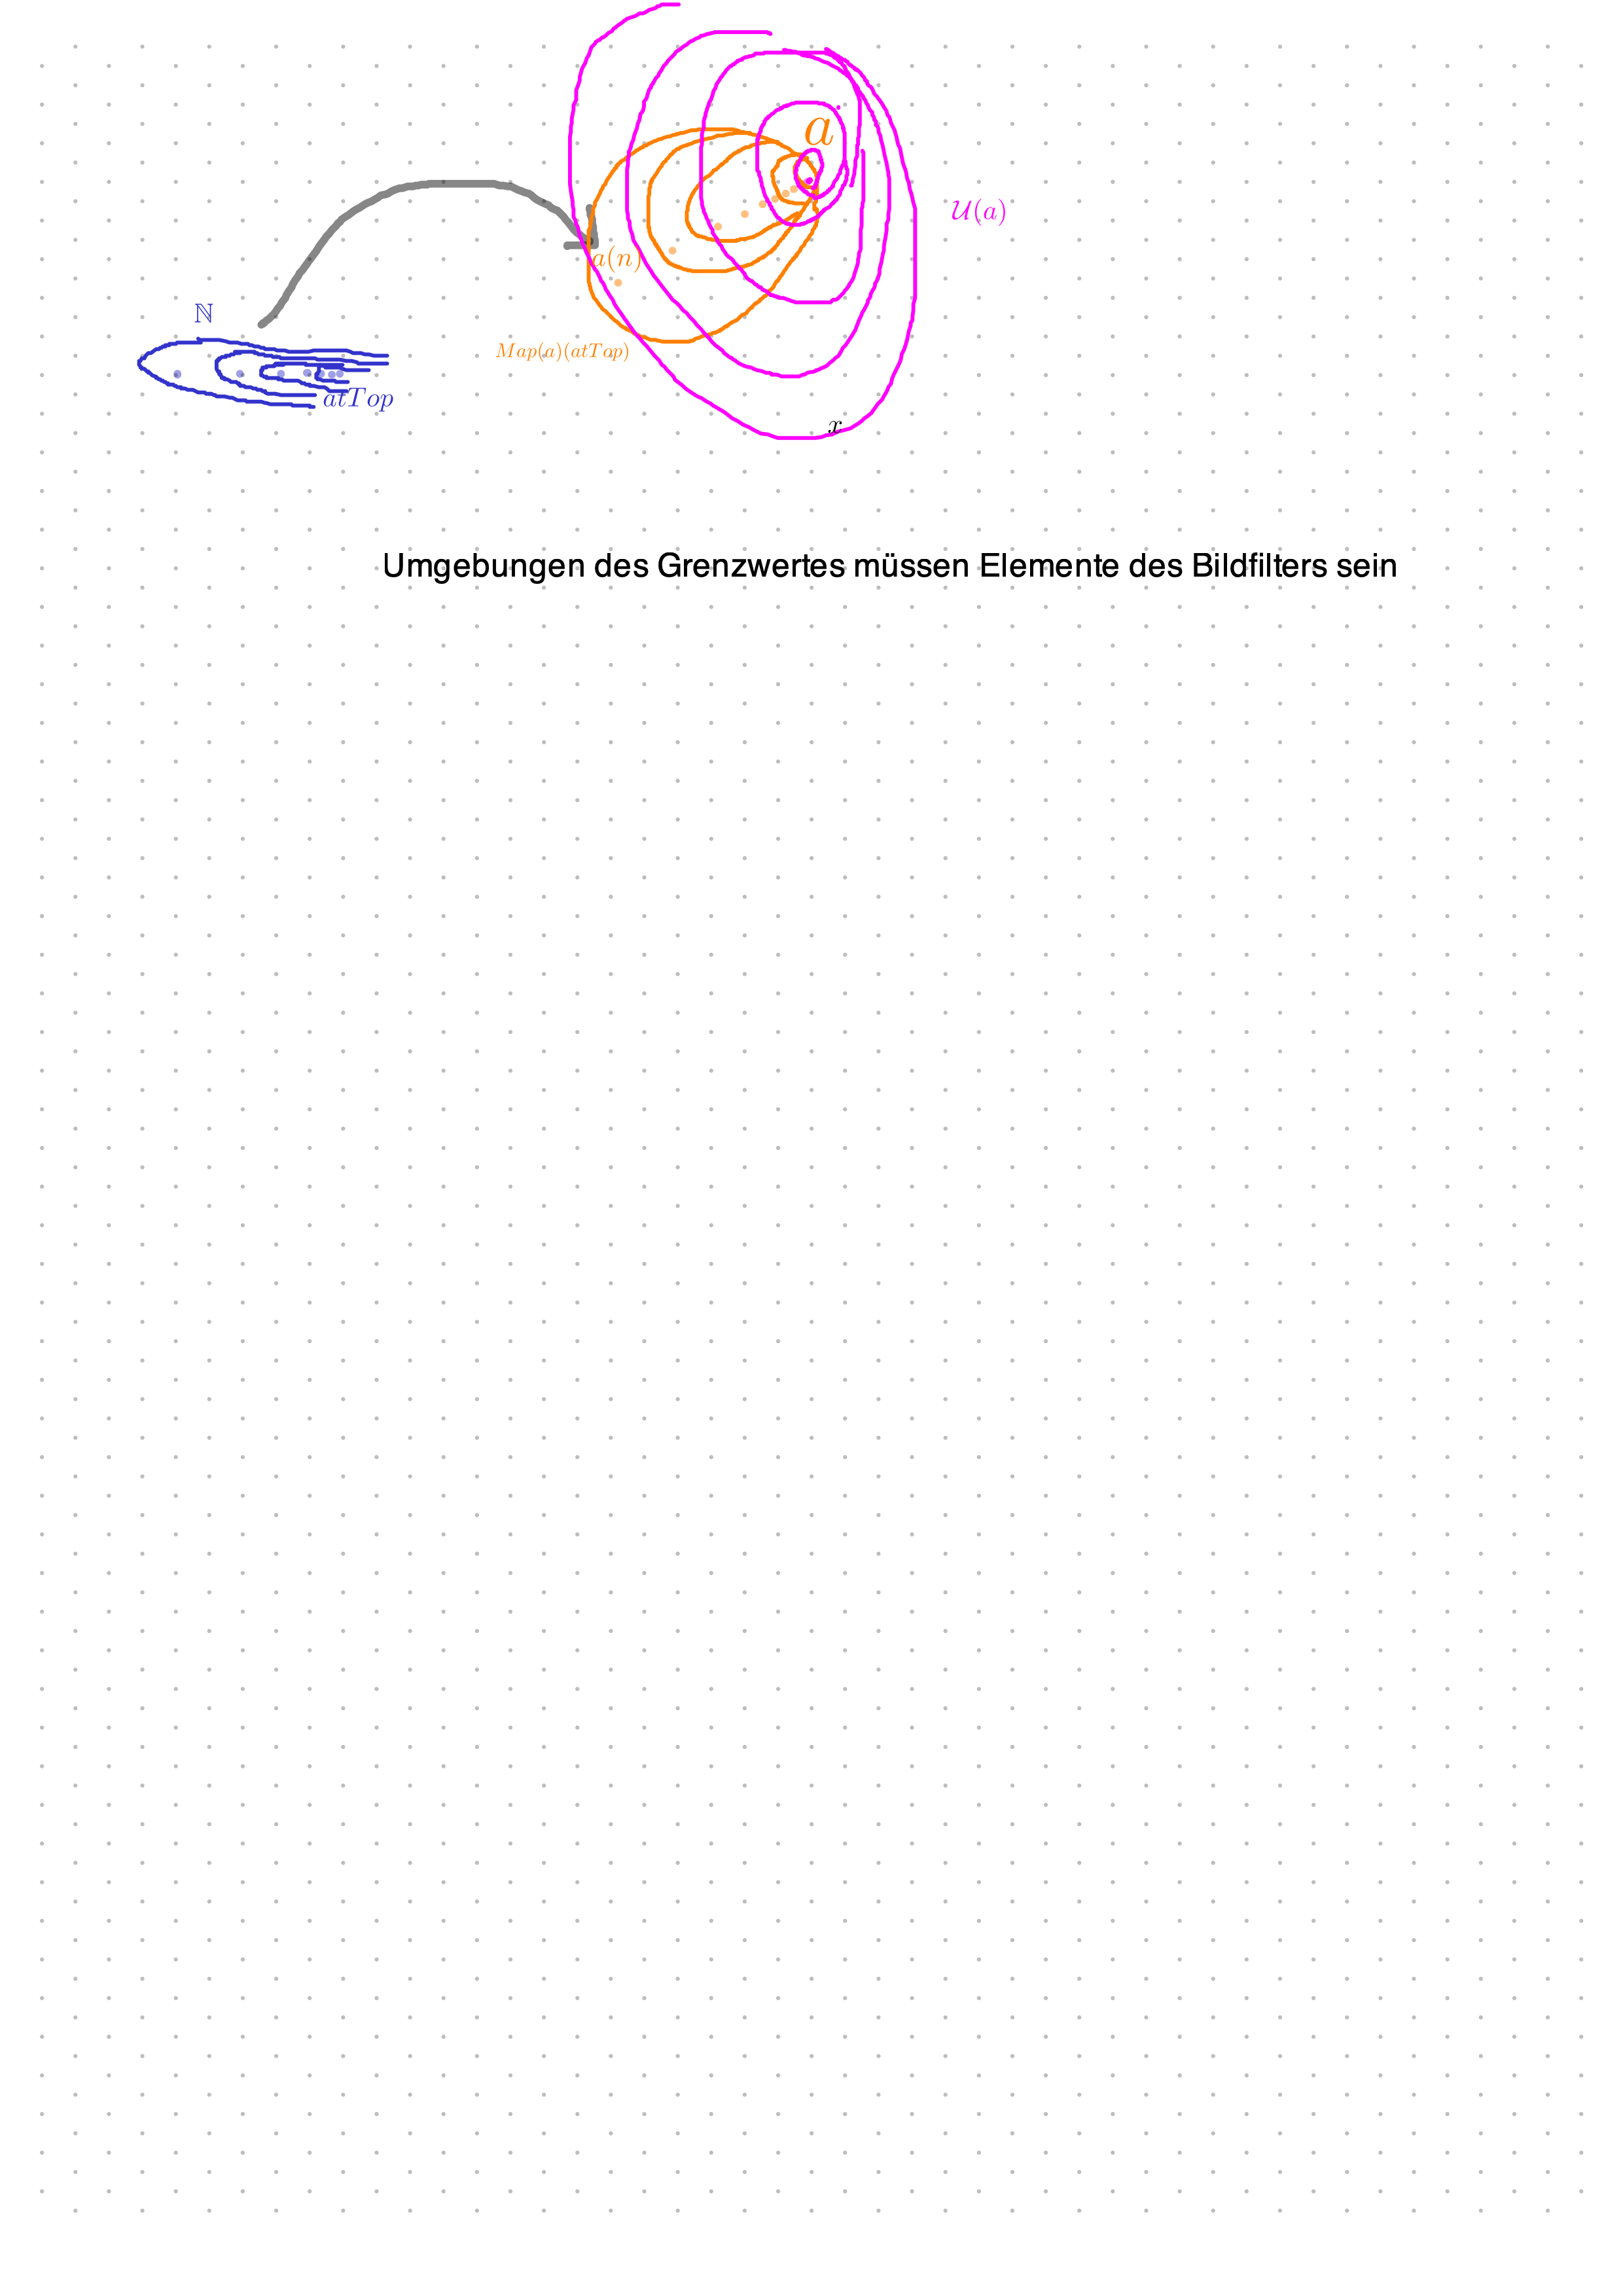
\includegraphics[width=1.1\textwidth]{images/filter_conv.png}
\end{figure}

\end{frame}


\end{document}

